\documentclass[a4paper,10pt]{article}
\usepackage{float}
\usepackage{graphicx}
\usepackage[ansinew]{inputenc}
\usepackage[spanish]{babel}
\usepackage{listings}
\usepackage{hyperref}
\usepackage{enumitem}
\usepackage{bookmark}
\inputencoding{latin1}
\graphicspath{/imagenes,/Casos de prueba}

\title{		\textbf{Trabajo Pr\'{a}ctico 0: \\
			Infraestructura b\'{a}sica
			}}

\author{	Fabrizio Cozza, \textit{Padr\'{o}n Nro. 97.402}                     \\
            \texttt{ fabrizio.cozza@gmail.com }                                              \\[2.5ex]
            Kevin Cajachu\'{a}n, \textit{Padr\'{o}n Nro. 98.725}                     \\
            \texttt{ kevincajachuan@hotmail.com }                                              \\[2.5ex]
            Luciano Giannotti, \textit{Padr\'{o}n Nro. 97.215}                     \\
            \texttt{luciano\_giannotti@hotmail.com.ar}                                              \\[3.5ex]
	 \newline
            \normalsize{1er. Cuatrimestre de 2018}                                      \\
            \normalsize{66.20 Organizaci\'{o}n de Computadoras  $-$ Pr\'{a}ctica Martes}  \\
            \normalsize{Facultad de Ingenier\'{i}a, Universidad de Buenos Aires}            \\
       }
\date{}


\begin{document}
\maketitle
\thispagestyle{empty}   % quita el n�mero en la primer p�gina
\newpage

\section{Objetivos}

Este Trabajo Pr\'{a}ctico tiene el fin de ayudarnos a familiarizarnos con las herramientas de software que utilizaremos posteriormente en otros trabajos, como es el emulador \textbf{gxemul} para correr programas sobre una maquina MIPS con el Sitema Operativo NetBSD.


\section{Programa}

El software de este trabajo esta escrito en lenguaje C y permite dibujar \textbf{Julia Sets} o \textbf{Conjuntos de Julia} segun los par\'{a}metros que le pasamos por l\'{i}nea de comando.
Estos parámetros son la region del plano complejo: delimitada por un centro, un ancho y un alto; una semilla que afectara el calculo para c\'{a}da pixel; la resoluci\'{o}n y la salida ya sea por pantalla o por archivo.
El formato a usar es  PGM o \textit{portable gray format}, que resulta \'{u}til para describir im\'{a}genes digitales en escala de grises.


\section{Implementaci\'{o}n}

Una vez recibidos los par\'{a}metros, para dibujar el Julia Set el programa obtiene de cada p\'{i}xel de la ventana a un punto en el plano complejo.
A ese punto se lo eleva al cuadrado y le suma la semilla mencionada en la secci\'{o}n anterior. Esto se repite hasta que el valor absoluto del resultado sea menor a 2, en cuyo caso se toma la cantidad de iteraciones y se imprime en el archivo PGM, representando el nivel de blanco de ese pi\'{i}xel.

Implementamos la clase \textbf{complex} para representar los numeros complejos.

Tambi\'{e}n implementamos las siguientes funciones dentro del main.c para dibujar los conjuntos:


\begin{lstlisting}[frame=single]
complex addComplexNumbers(complex a,complex b)
\end{lstlisting}
Suma dos n\'{u}meros complejos.
\newline

\begin{lstlisting}[frame=single]
complex sqrComplex(complex a)
\end{lstlisting}
Calcula la ra\'{i}z cuadrada de un n\'{u}mero complejo.
\newline

\begin{lstlisting}[frame=single]
double absComplex(complex a)
\end{lstlisting}
Calcula el valor absoluto de un complejo.
\newline


\begin{lstlisting}[frame=single]
int isValidNumber(char* arg)
\end{lstlisting}
Verifica que los valores ingresados para el ancho y el alto de la imagen sean v\'{a}lidos.
De ser as\'{i} devuelve 1, caso contrario devuelve 0.
\newline

\begin{lstlisting}[frame=single]
int isValidRes(char* arg) 
\end{lstlisting}
Verifica que el valor ingresado para la resoluci\'{o}n sea v\'{a}lido.
De ser as\'{i} devuelve 1, caso contrario devuelve 0.
\newline

\begin{lstlisting}[frame=single]
int isValidComplex(char* arg)
\end{lstlisting}
Verifica que el valor ingresado para el centro sea v\'{a}lido.
De ser as\'{i} devuelve 1, caso contrario devuelve 0.
\newline


\begin{lstlisting}[frame=single]
int processImage(int resW, int resH,
                 complex pPos, complex seed,
                 double w, double h,
                 FILE* im, int N)
\end{lstlisting}
Contiene la l\'{o}gica del dibujo de los sets. Recibe el alto y ancho de la misma, el centro, la semilla, la resoluci\'{o}n y la cantidad de iteraciones m\'{a}ximas.
Cada p\'{i}xel dentro de la resoluc\'{i}on ingresada es uno por uno transformado a n\'{u}meros complejos teniendo en cuenta el ancho y alto y el centro y se procesa el nivel en la escala de grises correspondiente a ese p\'{i}xel como se explica al principio de la secci\'{o}n.
Estos niveles se escriben en un buffer y luego en un archivo siguiendo el formato PGM.
La funci\'{o}n retorna -1 si ocurri\'{o} alg\'{u}n error.
\newline





El programa se compila con el siguiente comando:
\begin{lstlisting}[frame=single]
$gcc main.c -o tp0 -lm -std=gnu99
\end{lstlisting}

\section{C\'{o}digo C}

En esta secci\'{o}n colocaremos el c\'{o}digo fuente del programa en lenguaje C.

\lstinputlisting[basicstyle=\ttfamily\scriptsize,breaklines=true]{main.c}

\newpage

\section{Pruebas}

Para las pruebas compilamos el programa con gcc de la siguiente manera:

\begin{lstlisting}[frame=single]
$gcc main.c -o tp0
\end{lstlisting}
Luego corremos el archivo \textbf{test.sh}.
Ya que las pruebas son sobre las imágenes, las vamos a realizar a ojo comparandolas con las del enunciado y con las obtenidas en un generador online (\url{http://usefuljs.net/fractals/}).

Cabe destacar que las imagenes del generador tienen mayor rango dinamico que las del enunciado y nosotros decidimos generarlas como en \'{e}ste \'{u}ltimo.

Las imagenes obtenidas por nuestro trabajo se encuentran tambi\'{e}n en formato PNG en la subcarpeta \textit{imagenes}.
A su vez las imagenes del generador online se encuentran en \textit{Casos de prueba}.

\subsection{Caso con los valores por defecto}
Se obtiene una imagen como la primera figura del enunciado:

\begin{lstlisting}[frame=single]
$./tp0 -o uno.pgm
\end{lstlisting}

\begin{figure}[H]
\begin{center}
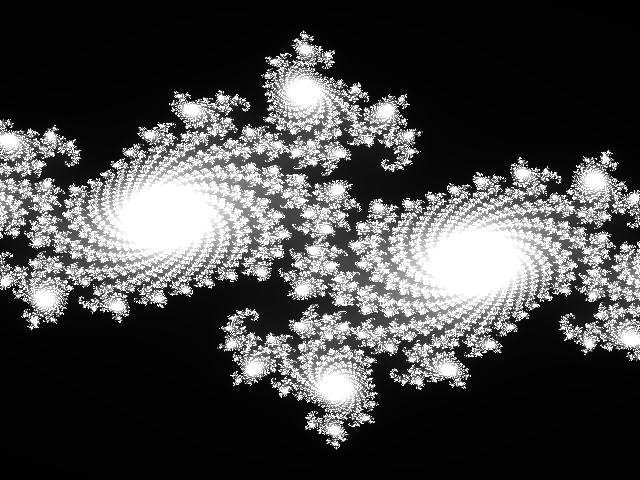
\includegraphics[width=0.5\textwidth]{imagenes/uno.png}
\caption{} \label{uno}
\end{center}
\end{figure}

\newpage

\subsection{Caso de imagen con zoom y otro centro}
Se obtiene una imagen como la segunda figura del enunciado:

\begin{lstlisting}[frame=single]
$ ./tp0 -c 0.282-0.007i -w 0.005 -H 0.005 -o dos.pgm
\end{lstlisting}

\begin{figure}[H]
\begin{center}

\includegraphics[width=0.5\textwidth]{imagenes/dos.png}
\caption{} \label{dos}
\end{center}
\end{figure}

\subsection{Caso de imagen con ancho 1 y centro 1}
Se obtiene una imagen como la primera del enunciado pero con un zoom x2 aplicado.
Realizamos esta prueba por ser un caso muy facil de reproducir y comprarar con otro generador de Julia Sets.

\begin{lstlisting}[frame=single]
$ ./tp0 -w 1 -H 1 -o tres.pgm
\end{lstlisting}

\begin{figure}[H]
\begin{center}
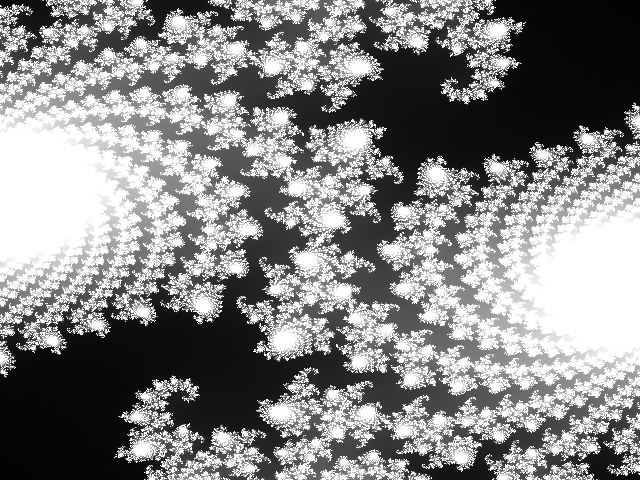
\includegraphics[width=0.5\textwidth]{imagenes/tres.png}
\caption{} \label{tres}
\end{center}
\end{figure}

\newpage

\subsection{Caso de imagen muy chica}

Imprimimos una imagen de 8x6 para que se puedan notar claramente los pixeles en la pantalla al hacer zoom con GIMP.

\begin{lstlisting}[frame=single]
$ ./tp0 -r 8x6 -o cuatro.pgm
\end{lstlisting}

\begin{figure}[H]
\begin{center}

\includegraphics[width=0.5\textwidth]{imagenes/cuatro.png}
\caption{} \label{cuatro}
\end{center}
\end{figure}

\subsection{Caso de imagen con otra semilla}

Esta imagen usa una semilla con sus dos componentes negativas y la imaginaria mucho mas grande que la real.
Esto es para comprobar que el centrado funcione correctamente, mas alla del caso del enunciado.
\begin{lstlisting}[frame=single]
$ ./tp0 -s -0.157-1.041i -o cinco.pgm
\end{lstlisting}

\begin{figure}[H]
\begin{center}

\includegraphics[width=0.5\textwidth]{imagenes/cinco.png}
\caption{} \label{cinco}
\end{center}
\end{figure}

\newpage

\subsection{Caso de imagen muy angosta}
En este caso cambiamos la resolucion para obtener una imagen de un pixel
de alto y 800 de ancho. \newline
Esto se realizo para verificar que no ocurren problemas de dibujado en casos extremos.
Es dif\'{i}cil observarla en el informe por lo que decidimos no colocarla. Sin embargo el archivo se encuentra en la misma carpeta del TP con el nombre \textit{seis.pgm}.

\begin{lstlisting}[frame=single]
$ ./tp0 -r 800x1 -o seis.pgm
\end{lstlisting}

\section{C\'{o}digo S}

En esta secci\'{o}n colocaremos el ci\'{o}digo assembly MIPS generado por NetBSD.

%\lstinputlisting[basicstyle=\ttfamily\scriptsize,breaklines=true]{main.s}

\section{Bibliograf\'{i}a}
\begin{enumerate}
\item GXemul. \\ http://gavare.se/gxemul/.
\item The NetBSD project. \\
	http://www.netbsd.org/.
\item http://es.wikipedia.org/wiki/Conjunto\_de\_Julia (Wikipedia).
\item PGM format specification.\\
	http://netpbm.sourceforge.net/doc/pgm.html.
\item Generador de fractales. \\
	http://usefuljs.net/fractals/
\item GIMP. \\
	https://www.gimp.org/
\end{enumerate}

\end{document}
